\section{Performance Evaluation}
In this section, we conduct extensive simulations to evaluate \emph{AutoPlan} by comparing with state-of-the-art works.

\textbf{Parameters.}
We select a $1210~\text{m}\times 1138~\text{m}$ campus area at the University of Nebraska–Lincoln, i.e., the deployment region $\mathcal{A}$. There are $K=127$ objects (i.e., buildings) in this region.
We obtain the scene geometry from OpenStreetMap3D and derive the feasible deployment region $\mathcal{F}\subseteq\mathcal{A}$ by extracting the union of building footprints. 
One existing private 5G base station is located near the southwest corner of $\mathcal{A}$, yielding the initial BS set $\hat{\mathcal{B}}={(\hat{x}_m,\hat{y}_m)}_{m=1}^{M}$ with $M=1$.
In the region $\mathcal{A}$, we collect $ P = 1494$ RSRP measurements $\hat{\mathbf r}=[\hat r_1,\hat r_2,\ldots,\hat r_P]$ via drive testing, with a 5G dongle (Quectel RM520N-GL).
The accurate location of the reciver is obtained by using RTK-GNSS, providing horizontal accuracy better than $2$ cm. 
For the deploy base stations, they are with a planar antenna array configured as a $1 \times 2$ horizontal linear array, with half-wavelength spacing between elements. 
The array adopts the 3GPP TR 38.901 directional antenna pattern and vertical polarization, representing a typical 5G small cell configuration. 
In the evaluation, we aim to select $N=5$ additional BS locations from the feasible region, i.e., $\bar{\mathcal{B}}={(\bar{x}_n,\bar{y}_n)}_{n=1}^{5}\subseteq\mathcal{F}$. 
To calculate coverage, we set $r_{th} = -90 \mathrm{dBm}$ and $a = 0.2, \mathrm{m}$.
The default maximum transmission power of the base station is $43\,\mathrm{dBm}$. Additionally, we set $\alpha = 10$ to balance the contributions of coverage and capacity in the target objective.
All simulations were conducted on a desktop with an Intel Core i7 CPU, an NVIDIA RTX 3080 GPU, and Ubuntu 24.04 OS, using Sionna RT v1.1.0~\cite{hoydis2023sionna}. 
Specifically, we calculate the RSRP and SNR by using \emph{RadioMapSolver} on a uniform $0.2,\mathrm{m}\times 0.2,\mathrm{m}$ grid.
To learn the building materials, we use the Adam optimizer~\cite{kingma2014adam} with learning rate $\eta=0.01$, for $E=300$ epochs. 
% Material parameters are initialized within physically feasible ranges (e.g., relative permittivity $\epsilon=3.5$ and conductivity $\sigma=0.2\mathrm{S/m}$). 

% \begin{figure}[!h]
% \centering
% 	\includegraphics[width=3.0in]{fig2.pdf}
% 	\caption{The trajectory of measured RSRP.}
% 	\label{fig:figure2}
% \end{figure}

We compare \emph{AutoPlan} with the following methods:
\begin{itemize}
\item \textbf{\emph{Random Sampling (RS).}} At each selection step, we randomly sample feasible candidate locations from $\mathcal{F}$ and evaluate $T(\cdot)$ using the calibrated DRT. For a fair comparison with \emph{AutoPlan}, we use the same pool of 100 candidate BS groups and report the group with the largest objective as the final solution.
\item \textbf{\emph{Exhaustive Search (ES).}} ES discretizes the feasible action space $\mathcal{F}$ using a $5~\mathrm{m}$ step factor, evaluates the objective $T(\cdot)$ at every candidate point under the calibrated DRT, and selects the location with the highest performance. 
ES provides a near-optimal result under the given resolution with the highest computational complexity.
\end{itemize}

\subsection{Digital Radio Twinning}
In this subsection, we evaluate the DRT for all the attributes of fidelity, tractability, and synchronicity, under the \emph{AutoPlan} algorithm.
Specifically, we collect the field measurement via a drive test in the City Campus of the University of Nebraska-Lincoln, as shown in Fig.~\ref{fig:figure2}. 


% \begin{figure}[!t]
% \centering
% 	\includegraphics[width=3.4in]{fig4.pdf}
% 	\caption{Mean square error (MSE) loss of DRT calibration.}
% 	\label{fig:figure4}
% \end{figure}

% \begin{figure*}[!t]
%   \centering
%   \subfigure[MSE loss]{
%     \includegraphics[width=0.25\textwidth]{fig3_1.pdf}
%   } 
%   \subfigure[Conductivity of building materials]{
%     \includegraphics[width=0.25\textwidth]{fig3_2.pdf}
%   }
%     \subfigure[Relative permittivity of building materials]{
%     \includegraphics[width=0.25\textwidth]{fig3_3.pdf}
%   }
%   % \subfigure[Original DRT and ES]{
%   %   \includegraphics[width=0.23\textwidth]{fig7_2.pdf}
%   % }
%   \caption{The MSE loss during DRT calibration, and conductivity, and relative permittivity of building materials.}
% \label{fig:figure3}
% \end{figure*}


\begin{figure*}[!t]
  \captionsetup{justification=centering}
  \centering
  \begin{minipage}[t]{0.24\textwidth}
    \centering
    \includegraphics[width=\linewidth]{fig2.pdf}
    \caption{The trajectory of measured RSRP.}
    \label{fig:figure2}
  \end{minipage}
  \hfill
  \begin{minipage}[t]{0.24\textwidth}
    \centering
    \includegraphics[width=\linewidth]{fig3_1.pdf}
    \caption{The MSE loss during DRT calibration.}
    \label{fig:fig3_1}
  \end{minipage}
  \hfill
  \begin{minipage}[t]{0.24\textwidth}
    \centering
    \includegraphics[width=\linewidth]{fig3_2.pdf}
    \caption{Conductivity of building materials, during DRT calibration.}
    \label{fig:fig3_2}
  \end{minipage}
  \hfill
  \begin{minipage}[t]{0.24\textwidth}
    \centering
    \includegraphics[width=\linewidth]{fig3_3.pdf}
    \caption{Relative permittivity of building materials, during DRT calibration.}
    \label{fig:fig3_3}
  \end{minipage}
\end{figure*}

As shown in Fig. 3, the training MSE loss steadily decreases over the 300 gradient descent steps and converges after around 200 steps, with a final minimum value of $113.78$. In other words, the sim-to-real discrepancy is reduced by $11.23 (8.98\%)$, by calibrating the parameters of building materials.

Note that it is impossible to reduce the MSE loss to zero, because the sim-to-real discrepancy is attributed to multiple complex factors, including but not limited to building materials, simulator abbreviation, radio propagation models, etc., losses, circuit noises, and much more. In our hardware setups, the time consumption of a single gradient descent step is $4.97 \mathrm{s}$ on average, with the variance of $0.07$. This indicates that, with sufficient GPU resources, the DRT can be continuously calibrated and updated in real time.

\vspace{0.8 em}
\begin{table}[!h]
\renewcommand\arraystretch{1.0}
    \caption{DRT inference time.} \centering
    \label{tab:TableI} 
	\setlength{\tabcolsep}{2.5mm}{
	\begin{tabular}{cccccc}
		\toprule
		%\diagbox{Data}{Error(\%)}{Function}& ReLU & Sigmoid & Linear\\ [3pt]
		Number of BSs & 1 & 2 & 3 & 4 & 5 \\ %[3pt]
		\midrule
		Avg. time ($\mathrm{s}$) & 0.39 & 0.72 & 0.87 & 1.07 & 1.24 \\
 
		\bottomrule
	\end{tabular}}
\end{table}
\vspace{0.8 em}

In addition, Table~\ref{tab:TableI} reports the inference time of the DRT under different numbers of deployed base stations. Notably, the average inference time is $0.39\mathrm{s}$ with a single base station and increases to $1.24 \mathrm{s}$ when five base stations are deployed, highlighting the computational cost associated with large-scale evaluations.

\subsection{Automatic Network Planning}
In this subsection, we evaluate the network performance of network planning under all comparison solutions. 

% Balancing performance gains against transmit power, we adopt $43\,\mathrm{dBm}$ as the default setting in subsequent experiments. This level yields the highest observed coverage and aligns with typical micro–base-station configurations.
% \begin{figure}[!h]
% \centering
% 	\includegraphics[width=3.0in]{fig4.pdf}
% 	\caption{Network performance under different methods.}
% 	\label{fig:figure4}
% \end{figure}

\begin{figure}[!t]
  \captionsetup{justification=centering}
  \centering
  \begin{minipage}[t]{0.24\textwidth}
    \centering
    \includegraphics[width=\linewidth]{fig4.pdf}
    \caption{Network performance under different methods.}
    \label{fig:figure4}
  \end{minipage}\hfill
  \begin{minipage}[t]{0.24\textwidth}
    \centering
    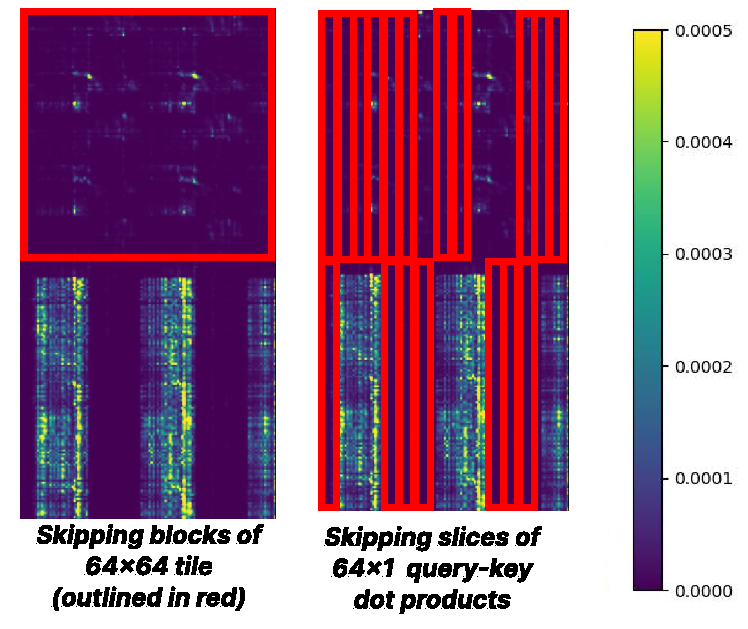
\includegraphics[width=\linewidth]{fig5.pdf}
    \caption{Network performance under different TX powers.}
    \label{fig:figure5}
  \end{minipage}
\end{figure}

The network performance, as defined in Eq.\ref{eq:eq3}, for all compared network planning methods is illustrated in Fig.\ref{fig:figure4}. 
As we can see, exhaustive search yields the highest overall performance, while random sampling performs significantly worse than both \emph{AutoPlan} and ES. 
Notably, \emph{AutoPlan} achieves performance nearly identical to that of ES, demonstrating its effectiveness in accurate and efficient BS deployment. In terms of computation time, ES requires $602$ minutes, approximately $58.33$ times longer than \emph{AutoPlan}, highlighting the latter’s practical efficiency.

\vspace{0.8 em}
\begin{table}[!h]
\renewcommand\arraystretch{1.0}
    \caption{Performance of deployment methods.} \centering
    \label{tab:TableII} 
	\setlength{\tabcolsep}{2.5mm}{
	\begin{tabular}{cccc}
		\toprule
		%\diagbox{Data}{Error(\%)}{Function}& ReLU & Sigmoid & Linear\\ [3pt]
		{ }& AutoPlan & ES & Random sampling \\ %[3pt]
		\midrule
		Coverage ($\%$) & \textbf{86.04} & 83.78 & 80.33 \\
		Capacity (bit/s/Hz) & 8.04 & \textbf{8.32} & 6.54\\
        Target & 16.64 & \textbf{16.70} & 14.57\\ 
		\bottomrule
	\end{tabular}}
\end{table}
\vspace{0.6 em}

In Table~\ref{tab:TableII}, we further show the detailed network coverage and capacity under 5 additional base station deployments. 
We can see that, \emph{AutoPlan} achieves 99.64\% overall target performance of ES, including a slightly higher network coverage ($2.40\%$), but a lower network capacity ($3.36\%$). These results demonstrate the effectiveness of \emph{AutoPlan} in selecting near-optimal BS deployment with significantly reduced computational cost.


% \begin{figure*}[!t]
%   \centering
%   \subfigure[AutoPlan]{
%     \includegraphics[width=0.3\textwidth]{fig7_1.pdf}
%   }
%   \subfigure[Random Sampling]{
%     \includegraphics[width=0.3\textwidth]{fig7_2.pdf}
%   }
%   \subfigure[Exhaustive Search]{
%     \includegraphics[width=0.3\textwidth]{fig7_3.pdf}
%   }
%   \caption{RSRP heatmaps of different network planning solutions, under calibrated digital radio twin.}
%   \label{fig:figure7}
% \end{figure*}


\begin{figure*}[!t]
  \captionsetup{justification=centering}
  \centering
  \begin{minipage}[t]{0.24\textwidth}
    \centering
    \includegraphics[width=\linewidth]{fig7_1.pdf}
    \caption{RSRP heatmaps of \emph{AutoPlan}.}
    \label{fig:fig7_1}
  \end{minipage}
  \hfill
  \begin{minipage}[t]{0.24\textwidth}
    \centering
    \includegraphics[width=\linewidth]{fig7_2.pdf}
    \caption{RSRP heatmaps of Random Sampling.}
    \label{fig:fig7_2}
  \end{minipage}
  \hfill
  \begin{minipage}[t]{0.24\textwidth}
    \centering
    \includegraphics[width=\linewidth]{fig7_3.pdf}
    \caption{RSRP heatmaps of Extensive Search.}
    \label{fig:fig7_3}
  \end{minipage}
  \hfill
  \begin{minipage}[t]{0.24\textwidth}
    \centering
    \includegraphics[width=\linewidth]{fig6.pdf}
    \caption{Base station locations of \emph{AutoPlan}.}
    \label{fig:figure6}
  \end{minipage}
\end{figure*}


% \begin{figure}[!t]
%   \captionsetup{justification=centering}
%   \centering
%   \begin{minipage}[t]{0.24\textwidth}
%     \centering
%     \includegraphics[width=\linewidth]{fig6.pdf}
%     \caption{Base station deployment locations of \emph{AutoPlan}, under original and calibrated DRT.}
%     \label{fig:figure6}
%   \end{minipage}\hfill
%   \begin{minipage}[t]{0.24\textwidth}
%     \centering
%     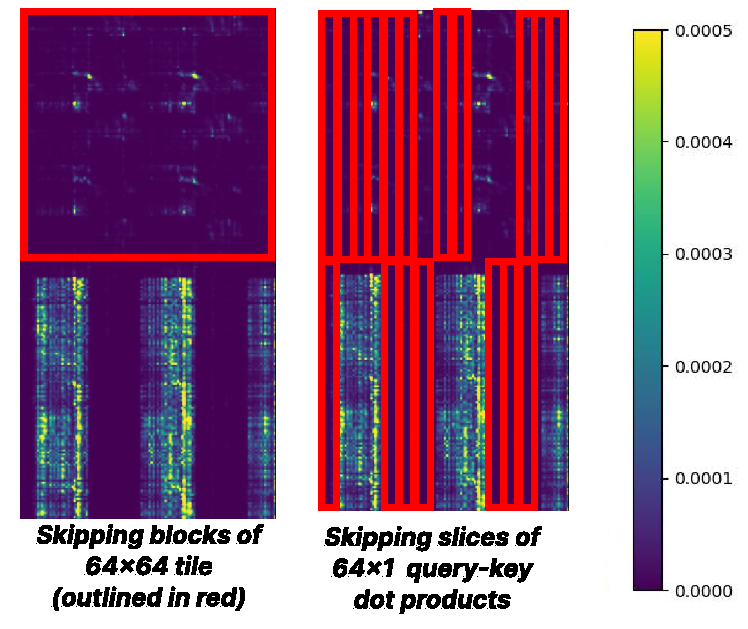
\includegraphics[width=\linewidth]{fig5.pdf}
%     \caption{Network performance under different transmission powers.}
%     \label{fig:figure5}
%   \end{minipage}
% \end{figure}


% \begin{figure}[!h]
% \centering
% 	\includegraphics[width=2.5in]{fig6.pdf}
% 	\caption{Base station deployment locations of \emph{AutoPlan}, under original and calibrated DRT.}
% 	\label{fig:figure6}
% \end{figure}

% \begin{figure}[!h]
% \centering
% 	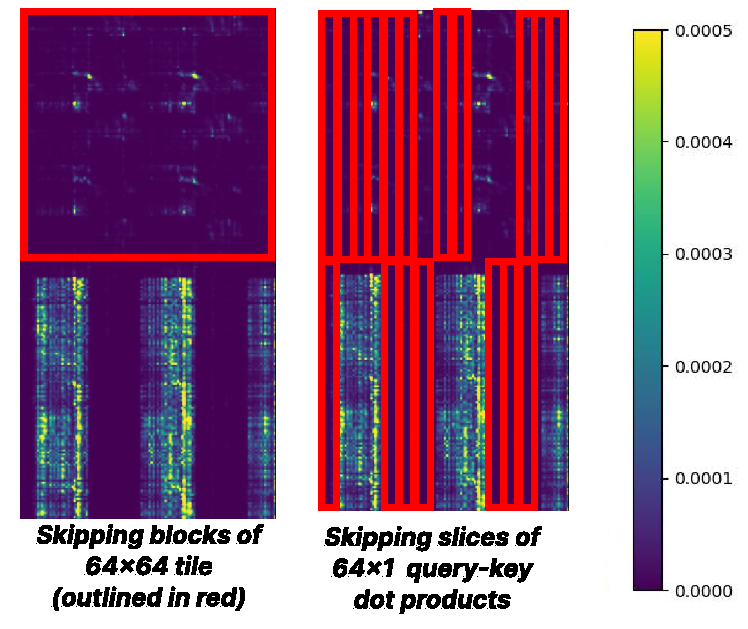
\includegraphics[width=3.0in]{fig5.pdf}
% 	\caption{Network performance under different methods.}
% 	\label{fig:figure5}
% \end{figure}


% In Fig.~\ref{fig:fig7_1}-\ref{fig:fig7_3}, we illustrate the final base station deployments and the resulted RadioMap. 
% It can be observed that the selected base station location of \emph{AutoPlan} is very similar with that of ES, which justifies its effectiveness and high sample efficiency.
In Fig.~\ref{fig:fig7_1}-\ref{fig:fig7_3}, we compare the RSRP heatmaps generated by the final BS deployments. 
Among the three methods, \emph{AutoPlan} achieves the largest coverage area with strong RSRP, while Random Sampling suffers from fragmented coverage and extensive low-signal regions. 
Moreover, four of the BSs selected by \emph{AutoPlan} are close to the placements in the ES solution, indicating that it can approximate the near-optimal deployment with far fewer evaluations. 


In Fig.~\ref{fig:figure6}, we show the impact of DRT on the selection of base station location under \emph{AutoPlan}. As observed, the deployment results obtained via the original DRT differ significantly from those based on the calibrated DRT, highlighting the influence of DRT accuracy on BS placement decisions. Quantitatively, the optimal deployment selected using \emph{AutoPlan} under the original DRT achieves a target value of $18.20$, while the same method applied on the calibrated DRT yields a target of $16.64$—indicating a gap of approximately $10\%$. This result underscores the necessity of calibrating the DRT to ensure reliable and accurate network planning decisions.

Moreover, we evaluate the sensitivity of coverage to transmit power in Fig.~\ref{fig:figure5}, which plots the coverage achieved by \emph{AutoPlan} as a function of the number of newly deployed BSs under different transmit power levels. As expected, coverage improves with increased power; however, the gain becomes marginal beyond $30,\mathrm{dBm}$. For example, when five new BSs are installed, increasing the power from $30,\mathrm{dBm}$ to $43,\mathrm{dBm}$ only results in an improvement of $2\%$. Considering the trade-off between performance and power consumption, we adopt $43,\mathrm{dBm}$ as the default setting in subsequent experiments. This value yields the highest observed coverage and corresponds to typical configurations of micro-base stations.

% After deploying five additional BSs, the resulting coverage, capacity, and overall performance are summarized in Table~\ref{tab:TableI}. Our proposed Bayesian Optimization (BO)-based method achieves $2.40\%$ higher coverage than Exhaustive Search (ES), with a $3.36\%$ lower capacity. Despite this trade-off, the resulting objective value $T(\cdot)$ is only $0.36\%$ lower than that of ES, indicating a negligible performance discrepancy while significantly reducing computational cost. Additionally, compared to the Heuristic baseline, our method achieves a $21.91\%$ improvement in the overall objective, clearly demonstrating the effectiveness of BO in identifying high-quality BS deployment configurations. These results validate the benefits of combining a calibrated digital twin with BO-based search: near-optimal performance with drastically fewer evaluations.


% comparison algorithms

% \begin{figure}[!t]
% \centering
% 	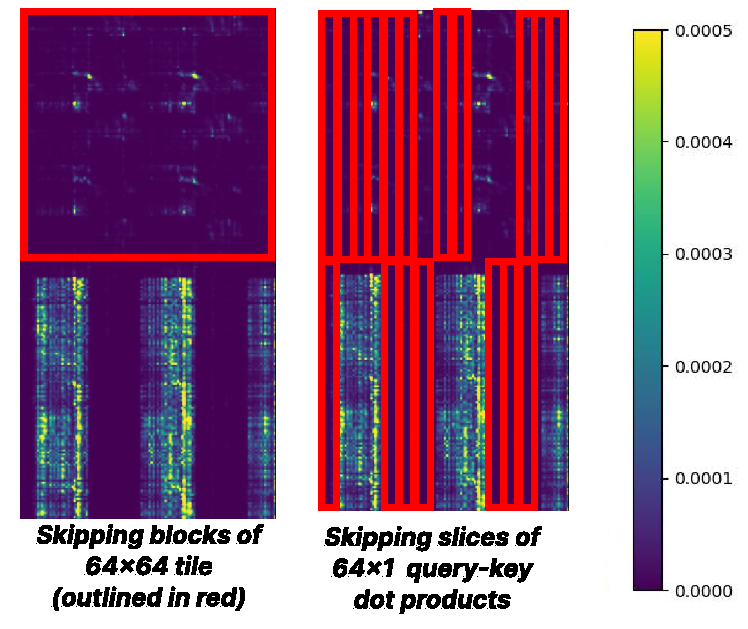
\includegraphics[width=3.3in]{fig5.pdf}
% 	\caption{Coverage of AutoPlan under different transmit powers.}
% 	\label{fig:figure5}
% \end{figure}


% overall performance


% scalability (tbd)


% tbd




% \begin{figure}[!t]
% 	\centering
% 	\includegraphics[width=2.6in]{fig/f_original_cost_history_perf_change_ratio.pdf}
% 	\vspace{-0.05in}\caption{\small The normalized performance under changing slice demands.}
% 	\label{fig:f_original_cost_history_perf_change_ratio}
% \end{figure}